\documentclass[a4paper,12pt]{article}
    
\usepackage{xltxtra}
\usepackage{polyglossia}
\usepackage{url}
\usepackage{graphicx}

\defaultfontfeatures{Ligatures=TeX,Mapping=tex-text}

\setmainfont{Liberation Serif}

\setromanfont{Liberation Serif} 
\setsansfont{Liberation Sans} 
\setmonofont{Nimbus Mono PS} 
\newfontfamily\cyrillicfonttt{Nimbus Mono PS}

\setdefaultlanguage{russian}
\setlength{\parindent}{0pt}
\urlstyle{rm}
\graphicspath{{img/}}
\DeclareGraphicsExtensions{.pdf,.png,.jpg}

\title{Формула Джеффа Таппера}
\author{Станислав Смирнов}

\begin{document}
\maketitle

\section{Введение}
\subsection{Общие сведения}
\begin{equation}\label{eq:tupper}
  \frac{1}{2} \: < \: \left\lfloor \mathrm{mod}\: \left( \left\lfloor \frac{y}{17} \right\rfloor \: 2^{-17 \lfloor x \rfloor - \mathrm{mod} \left( \lfloor y \rfloor, \: 17 \right)} ,\: 2 \right) \right\rfloor
\end{equation}

Джефф Таппер в 2001 году опубликовал свою (1) формулу, которую потом назвали самореферентной. Что это значит? При определенных условиях, а именно
\texttt{y=4 858 450 636 189 713 423 582 095 962 494 202 044 581 400 587 983 244 549 483 093 085 061 934 704 708 809 928 450 644 769 865 524 364 849 997 247 024 915 119 110 411 605 739 177 407 856 919 754 326 571 855 442 057 210 445 735 883 681 829 823 754 139 634 338 225 199 452 191 651 284 348 332 905 131 193 199 953 502 413 758 765 239 264 874 613 394 906 870 130 562 295 813 219 481 113 685 339 535 565 290 850 023 875 092 856 892 694 555 974 281 546 386 510 730 049 106 723 058 933 586 052 544 096 664 351 265 349 363 643 957 125 565 695 936 815 184 334 857 605 266 940 161 251 266 951 421 550 539 554 519 153 785 457 525 756 590 740 540 157 929 001 765 967 965 480 064 427 829 131 488 548 259 914 721 248 506 352 686 630 476 300}
на графике будет изображение самой формулы (см. Рисунок \ref{fig:selfref})\\

\begin{figure}[h]
\center{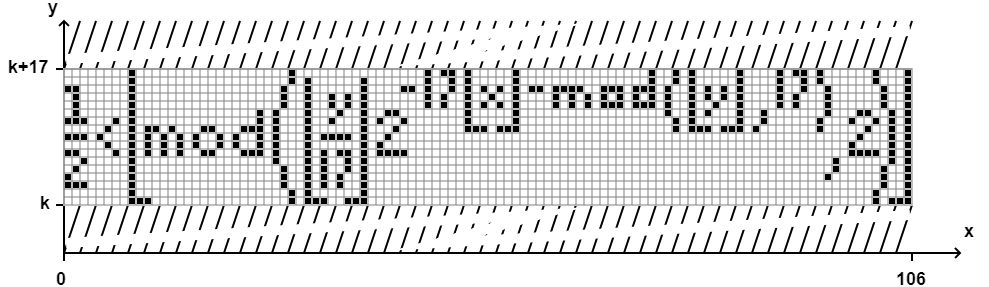
\includegraphics[scale=0.5]{selfref.png}}
\caption{Изображение неравенства (1) на графике этого неравенства}
\label{fig:selfref}
\end{figure}

Чем же таким занимался Джефф, что нашел такую формулу "всего"? Он разрабатывал программу GrafEq для построения графиков и опубликовал находку в своем докладе о надежных способах построения двумерных компьютерных графиков для SIGGRAPH. Из доклада можно догадаться, что Таппер был математиком и разрабатывал программы для построения графиков. Во всяком случае, про него достаточно мало информации в Интернете, ни когда он родился, ни чем он занимается, ни где живет\\

\subsection{О графике}
Изображение неравенства на графике этого же неравенства это еще не все, на этом графике можно найти любое изображение размером 106x17 пикселей, правда, черно-белое\\

Если построить этот график в какой-либо программе для построения графиков, например, Desmos\footnote{\url{https://www.desmos.com/calculator/oczhhtqnz6}}, то мы, конечно, можем пролистать до координат, где неравенство воспроизвело само себя, но это будет очень долго, мы можем посмотреть, например, на $y=17$, на этой координате закрашен квадрат от $(17, 0)$ до $(18, 1)$\\

\section{Математический смысл}
Вспомним неравенство, которое было показано в параграфе 1.1:
\begin{equation}\label{eq:tupper}
  \frac{1}{2} \: < \: \left\lfloor \mathrm{mod}\: \left( \left\lfloor \frac{y}{17} \right\rfloor \: 2^{-17 \lfloor x \rfloor - \mathrm{mod} \left( \lfloor y \rfloor, \: 17 \right)} ,\: 2 \right) \right\rfloor
\end{equation}

В нем могут быть понятны не все операторы, например, $\mathrm{mod}(x, y)$ или $\lfloor x \rfloor$:\\

$\mathrm{mod}(x, y)$ -- это остаток от деления $x$ на $y$, т.е.
\begin{equation}
  \mathrm{mod}(11, 5) = 1; 11=5\cdot2+1
\end{equation}

$\lfloor x \rfloor$ -- окргление к меньшему, т.е.
\begin{equation}
  \lfloor 0.5 \rfloor=0;
  \lfloor 0.9 \rfloor=0;
  \lfloor 1.1 \rfloor=1
\end{equation}
\section{Реализация в браузере}
Алгоритм генерации изображений на графике формулы Таппера давно известен:
\begin{enumerate} 
  \item Необходимо представить картинку как черно-белое растровое изображение разрешением 116 на 17 пикселей
  \item Сверху-вниз, слева-направо, заменить пустые клетки на 0, а закрашенные на 1
  \item Перевести число, которое мы получили, в десятичную систему счисления
  \item Разделить полученное число на 17
\end{enumerate}

Для реализации в браузере необходимо использовать JavaScript, отсюда вытекает несколько проблем:
\begin{enumerate} 
  \item Числа, с которыми умеет работать JS не превышают \texttt{9007199254740991}, а максимальное число в формуле Таппера во много раз больше
  \item В алгоритме выше нам необходимо проверить 1972 клетки на их состояние, закрашены они или нет. Но с данной проверкой происходит еще запись значения клетки в память, поэтому этот процесс достаточно медленный
  \item Реальный график. Никто не будет листать график до координат, где находится заветная картинка, поэтому я использовал готовое приложение для построения графиков и автоматически перемещаю к картинке, но, исходя из пункта 1 в данном списке, мы не может оперировать большими числами, поэтому график можно посмотреть всего до \texttt{y=999999976}
\end{enumerate}

Чтобы победить проблему №1, была использована библиотека, которая позволяет оперировать числами любой длины. К слову, в JS есть и встроеный тип BigInt, но его природа не позволяет передавать его как аргумент в другие функции, чтобы дальше использовать число\\

Для оформления проекта использовалась достаточно популярная библиотека Bootstrap 5 версии. Библиотека ничем не примечательна, она лишь дает некое упрощение, где не надо заморачиваться с дизайном\\

Так же, для операций с элементами на странице использовалась библиотека jQuery, она как и Bootstrap просто упрощает разработку\\

Принцип работы достаточно прост. Человек может отметить пиксели на полотне, которые он бы хотел закрасить, нажать кнопку и получить свое число k. В это же поле с числом k человек может ввести произвольное число и по нажатию на кнопку получить картинку\\

Слева расположена Справочная информация и пара примеров таких картинок, краткая справочная информация и ссылка на этот документ\\

\section{Вывод}
Формула Таппера это очень интересный феномен. Хоть она почти не имеет применения в современных реалиях, достаточно интересно разобраться в том, как она работает.\\

Для программиста это может быть неплохим проектом, где он научиться работать с большими числами, бинарными данными и сложными вычислениями\\

\renewcommand*{\refname}{\vspace*{-2em}}
\section{Список используемой литературы}
\begin{thebibliography}{9}
	\bibitem{q} Jeff Tupper, \emph{Reliable Two-Dimensional Graphing Methods
for Mathematical Formulae with Two Free Variables}, 2001.
	\bibitem{qq} Prathamesh Deshmukh, \emph{Transformation of the pixels in Tupper's self-referential formula}, 2018.
	\bibitem{qqq} Margaret Fortman, \emph{Tupper’s Self-Referential Formula}, 2015.
	\bibitem{qqqq} Numberphile, \emph{The ‘Everything′ Formula}, YouTube, 2015.
	\bibitem{qqqqq} Формула Таппера, \emph{\url{https://ru.wikipedia.org/wiki/Формула_Таппера}}, Wikipedia, 2021.
\end{thebibliography}
\end{document}